%!TeX root=../tese.tex
%("dica" para o editor de texto: este arquivo é parte de um documento maior)
% para saber mais: https://tex.stackexchange.com/q/78101

%% ------------------------------------------------------------------------- %%

% "\chapter" cria um capítulo com número e o coloca no sumário; "\chapter*"
% cria um capítulo sem número e não o coloca no sumário. A introdução não
% deve ser numerada, mas deve aparecer no sumário. Por conta disso, este
% modelo define o comando "\unnumberedchapter".
\chapter{Introduction}
\label{cap:introduction}

\enlargethispage{.5\baselineskip}

\section{Background}
Weather and climate predictions are recognized as a good for mankind,
due to the information they yield for diverse activities. 
For instance, short-range forecasts are useful for public use, while
medium-range forecasts are helpful for industrial activities and agriculture. 
Seasonal forecasts (one up to three months) are important to energy planning and agriculture.
At last, longer-range forecasts (one century, for instance) are useful for climate change 
projections that are important for government planning.

The first global Numerical Weather Prediction models emerged in the 1960s
with applications to weather, seasonal and climate forecasts. 
All these applications are essentially based on the same set of Partial Differential Equations
(PDEs) but with distinct time scales \citep{will:2007}. These PDEs are defined on the sphere
and model the evolution of the atmospheric fluid given the initial conditions.
One important component of global models is the dynamical core, which is responsible
for solving the PDEs that governs the atmosphere dynamics on grid-scale. 
The development of numerical methods for dynamical cores has been an active research area since the 1960s.

Global models use the sphere as the computational domain and therefore they require a discretization
of the sphere. 
The first global models used the latitude-longitude grid (Figure \ref{latlon-grid}), which is
very suitable for finite-differences schemes. The major drawback of the latitude-longitude grid
is the clustering of points at the poles, known as the ``pole problem'', which leads to extremely
small time steps for explicit-in-time schemes due to the Courant-Friedrichs-Lewy (CFL) condition, 
making these schemes computationally very expensive.

The most successful method adopted in global atmospheric dynamical cores that overcomes the CFL 
restriction is the Semi-Implicit Semi-Lagrangian (SI-SL) scheme \citep{randall:2018}, which 
emerged in the 1980s and consists of the Lagrangian advection scheme applied at each time-step 
and the solution of fast gravity waves implicitly, allowing very large time steps despite the pole problem.
The SI-SL approach combined with finite differences is still used nowadays, for instance in 
the UKMetOffice global model ENDGame \citep{wood:2014, benacchio:2016}.
The expensive part of the  SI-SL approach is to solve an elliptic equation at each time step,
that comes from the semi-implicit discretization, which requires global data communication,
being inefficient to run in massive parallel supercomputers. Besides that, 
Semi-Lagrangian schemes are inherently non-conservatives for mass,
which is critical for climate forecasts \citep{will:2007}.

\begin{figure}
  \centering
  \begin{subfigure}{.3\linewidth}
    \centering
    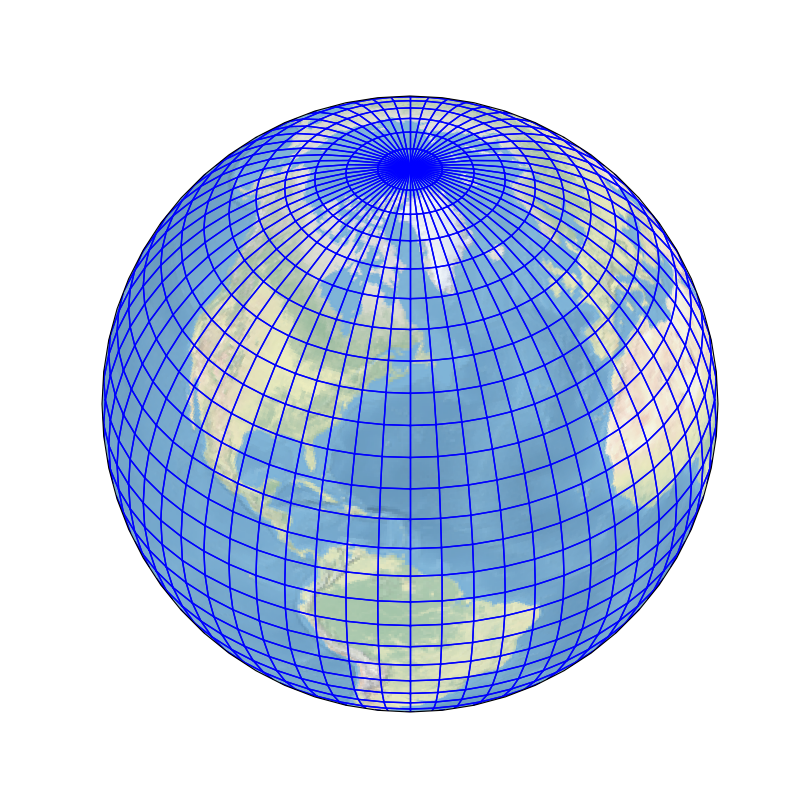
\includegraphics[width = \linewidth]{latlon_sphere}
      \caption{Latitude-longitude grid}\label{latlon-grid}
  \end{subfigure}%
  \hspace{1em}% Space between image A and B
  \begin{subfigure}{.3\linewidth}
    \centering
    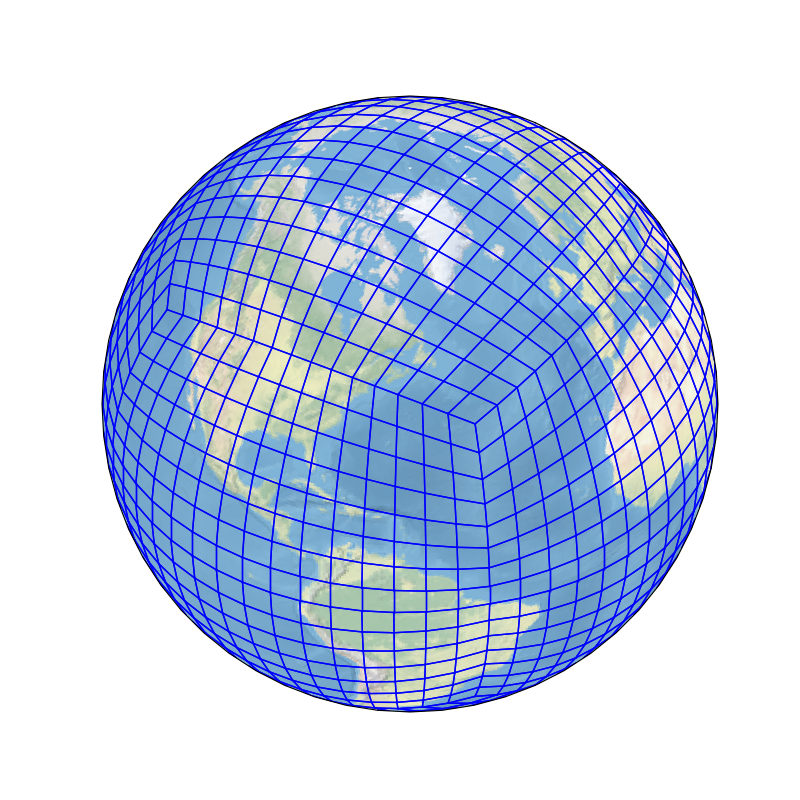
\includegraphics[width = \linewidth]{gnomonic_equiangular_15_sphere}
      \caption{Cubed-sphere}\label{cs-grid}
  \end{subfigure}%
  \hspace{2em}% Space between image B and C
  \begin{subfigure}{.3\linewidth}
    \centering
    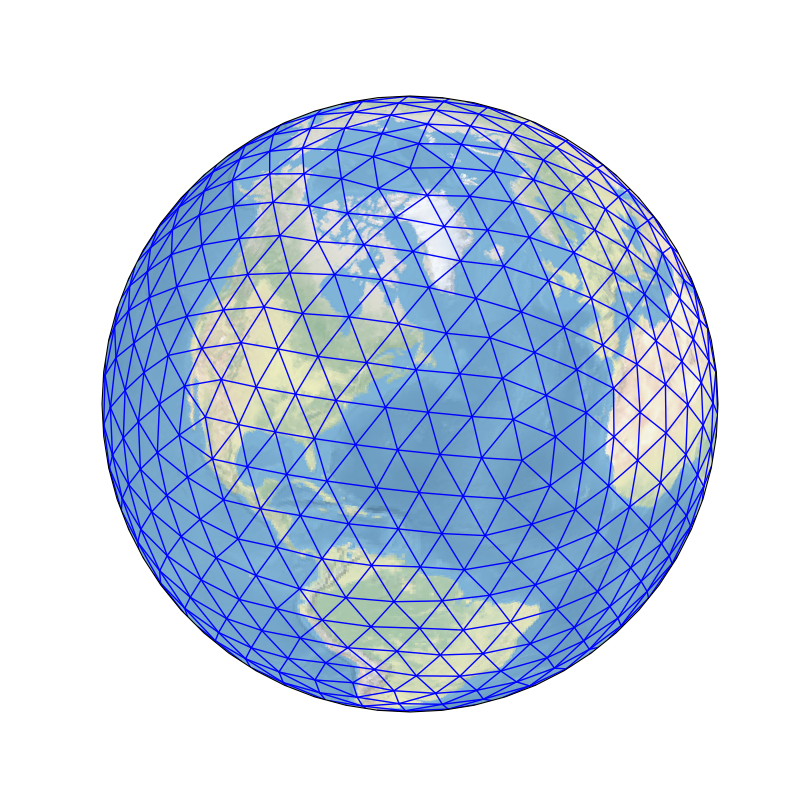
\includegraphics[width = \linewidth]{icos_pol_nopt_3_edsphere}
	  \caption{Icosahedral grid}\label{icos-grid}
  \end{subfigure}
  \begin{subfigure}{.3\linewidth}
    \centering
    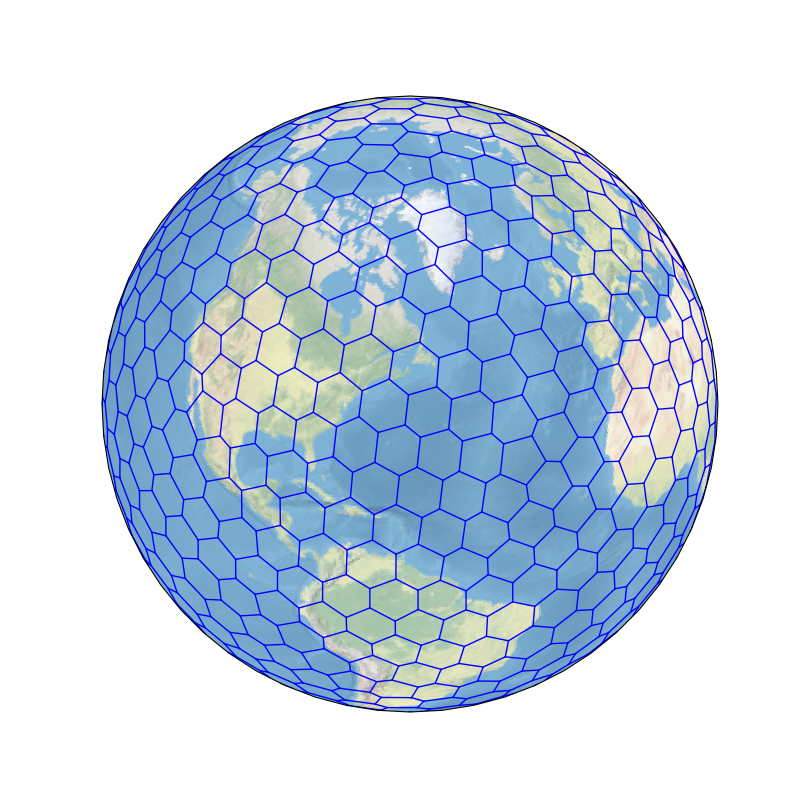
\includegraphics[width = \linewidth]{icos_pol_nopt_3_edhxsphere}
	  \caption{Pentagonal/Hexagonal grid}\label{voronoi-grid}
  \end{subfigure}
  \begin{subfigure}{.3\linewidth}
    \centering
    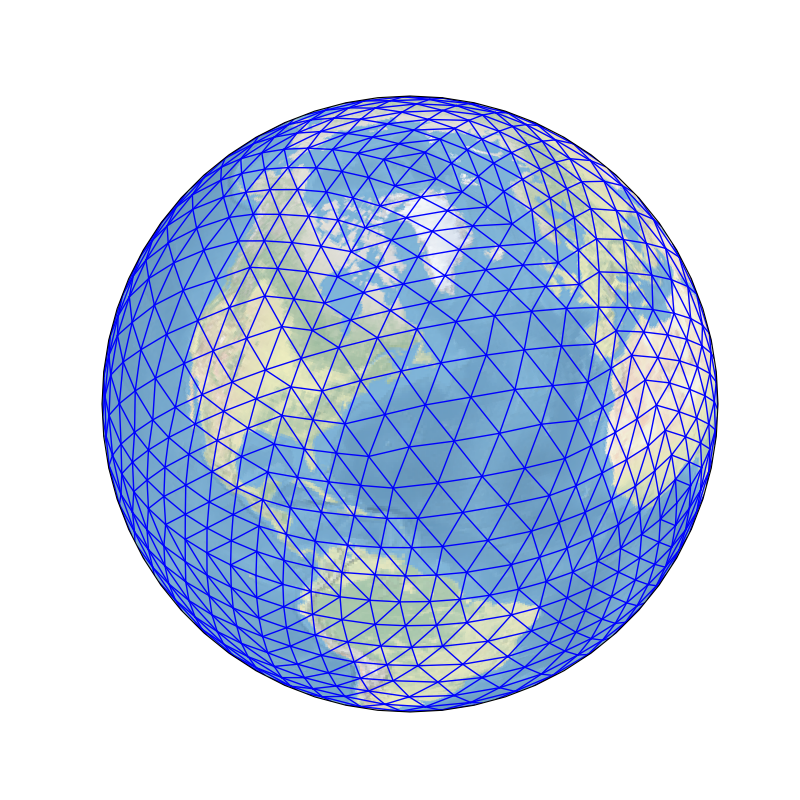
\includegraphics[width = \linewidth]{octg_pol_nopt_4_edsphere}
	  \caption{Octahedral grid}\label{octg-grid}
  \end{subfigure}
  \caption{Examples of spherical grids: latitude-longitude grid (a) and grids based on Platonic solids (b)-(d).}
\end{figure}

The emergence of the Fast Fourier Transform (FFT) in the 1960s with the work from 
\citet{cooley:1965} allowed the computation of discrete Fourier transforms with
$N\log(N)$ complexity. 
The viability of the usage of FFTs for solving atmospheric flows was shown by \citet{orszag:1970},
using the barotropic vorticity equation on the sphere, and by \citet{eliasen:1970}, using
the primitive equations.
The spectral transform method expresses latitude-longitude grid values, that represent some scalar field,
using truncated spherical harmonics expansions, which consists of Fourier expansions 
in latitude circles and Legendre functions expansions in longitude circles. 
The coefficients in the spectral expansions are known
as spectral coefficients and are usually thought to live in the so-called spectral space.
Given the grid values, the spectral coefficients are obtained by performing a FFT followed by a 
Legendre Transform (LT). 
Conversely, given the spectral coefficients,
the grid values are obtained by performing an inverse LT followed by an inverse FFT.
The main idea of the spectral method is to apply the spectral transform, in order to 
go the spectral space, and evaluate spatial derivatives in the spectral space, which
consists of multiplying the spectral coefficients by constants. 
Then, the method performs the inverse spectral transform
in order to get back to grid space, and the nonlinear terms are treated on the grid space
\citep{krishnamurti:2006}.

The spectral transform makes the use of SI-SL methods computationally cheap, 
since the solution to elliptic problems becomes easy, once the spherical harmonics are
eigenfunctions of the Laplacian operator on the sphere.
Therefore, the spectral transform method gets faster when combined with the SI-SL approach
due to the larger times-steps allowed in this case.
Due to these enhancements, the spectral transform dominated global atmospheric modeling 
\citep{randall:2018} since the 1980s.
Indeed, the spectral method is still used in many current operational Weather Forecasting models such as
the Integrated Forecast System (IFS) from  European Centre for Medium-Range Weather Forecasts (ECMWF),
Global Forecast System (GFS) from National Centers for Environmental Prediction (NCEP) and the
Brazilian Global Atmospheric Model (BAM) \citep{figueroa:16} from  Center for Weather Forecasting 
and Climate Research [Centro de Previsão de Tempo e Estudos Climáticos (CPTEC)].

With the beginning of the multicore era in the 1990s, the global atmospheric models
started to move towards parallel efficiency aiming to run at very high resolutions. 
Even though the spectral transform expansions have a global data dependency, some parallelization
is feasible among all the computations of FFTs, LTs and their inverses \citep{barros:1995}.
However, the parallelization of the spectral method requires data transpositions in order
to compute FFTs and LTs in parallel.  
These transpositions demand a lot of global communication using, for instance,
the Message Passing Interface (MPI) \citep{zheng:2018}. 
Indeed, the spectral transform becomes the most expensive component of global spectral models
when the resolution is increased due to the amount of MPI communications \citep{mueller:2019}.

The adiabatic and frictionless continuous equations that govern the atmospheric flow have 
conserved quantities. Among them, some of the most important are mass, total energy, 
angular momentum and potential vorticity \citep{thuburn:2011}.
As we pointed out, Semi-Lagrangian schemes lack mass conservation. Nevertheless, 
these schemes have been employed in dynamical cores for better computational performance.
However, dynamical cores should have discrete analogous of the 
continuous conserved quantities, especially concerning for longer simulation runs.

Aiming for better performance in massively parallel computers and conservation properties, 
new dynamical cores have been developed since the beginning of the 2000s.
Novel spherical grids have been proposed, in order to avoid the pole problem.
A popular choice are grids based on Platonic solids \citep{stan:2012}.
The construction of these grids relies on a Platonic circumscribed on the sphere and 
the projection of its faces onto the sphere, which leads to quasi-uniform and more isotropic
spherical grids.
Some examples of spherical grids based on Platonic solids employed in the new generation
of dynamical cores are the cubed-sphere (Figure \ref{cs-grid}), icosahedral grid (Figure \ref{icos-grid}), 
the pentagonal/hexagonal grid (Figure \ref{voronoi-grid}) and octahedral grid (Figure \ref{octg-grid}),
which are based on the cube, icosahedron, dodecahedron and octahedron, respectively \citep{ullrich:2017}.

TRSK \citet{thuburn:2009}, \citet{ringler:2010} 
MPAS example \citep{skamarock:12}. accuraccy \citep{weller:12, peixoto:13, peixoto:16}
\citep{santos:2021}.
